\documentclass[aspectratio=169,12pt,t]{beamer}

% --- Theme: Metropolis (modern, clean) ---
\usetheme[progressbar=frametitle,numbering=fraction,block=fill]{metropolis}

% --- Fira Sans font (install texlive-fonts-extra if missing) ---
\IfFileExists{FiraSans.sty}{\usepackage[sfdefault]{FiraSans}}{}

% --- Light background with warm accent ---
\definecolor{mDarkTeal}{RGB}{35,55,59}
\definecolor{mLightBrown}{RGB}{235,228,216}
\definecolor{mAccent}{RGB}{140,70,20}

\setbeamercolor{normal text}{fg=mDarkTeal,bg=white}
\setbeamercolor{alerted text}{fg=mAccent}
\setbeamercolor{frametitle}{bg=mDarkTeal,fg=white}
\setbeamercolor{progress bar}{fg=mAccent,bg=mLightBrown}
\setbeamercolor{title separator}{fg=mAccent}
\setbeamercolor{progress bar in head/foot}{fg=mAccent,bg=mLightBrown}
\setbeamercolor{progress bar in section page}{fg=mAccent,bg=mLightBrown}

% --- Packages ---
\usepackage[utf8]{inputenc}
\usepackage{amsmath,amssymb,amsthm}
\usepackage{mathrsfs}
\usepackage{tikz}
\usetikzlibrary{arrows.meta,positioning,calc,decorations.pathreplacing,shapes,patterns}
\usepackage{pgfplots}
\pgfplotsset{compat=1.18}

% --- TikZ diagram styles (shared across the series) ---
\tikzset{
  axisln/.style={-{Stealth[length=2.6mm]}, line width=0.8pt, gray!75},
  curveln/.style={line width=1.6pt, line cap=round, line join=round},
  projln/.style={dash pattern=on 2.6pt off 2pt, line width=0.7pt},
  guide/.style={-{Stealth[length=2.6mm,width=2.2mm]}, line width=1.1pt},
}
% point marker with a white halo: \dotpt{color}{(coord)}
\newcommand{\dotpt}[2]{%
  \fill[white] #2 circle (3.6pt);
  \fill[#1] #2 circle (2.4pt);
}
% open point marker: \opendotpt{color}{(coord)}
\newcommand{\opendotpt}[2]{%
  \fill[white] #2 circle (3.6pt);
  \draw[#1, line width=1pt] #2 circle (2.4pt);
}

% --- Semi-transparent white highlight for text on top of background images ---
\usepackage[most]{tcolorbox}

% Inline highlight: \hl{short text}
\newtcbox{\hl}{%
  nobeforeafter, tcbox raise base,
  colback=white, opacityback=0.6,
  colframe=white, opacityframe=0,
  sharp corners, boxsep=2pt, left=3pt, right=3pt, top=2pt, bottom=2pt%
}

% Block highlight: \begin{hlbox} ... \end{hlbox}  (multi-line, paragraphs, itemize)
% Optional argument accepts any tcolorbox key, e.g. [width=0.6\linewidth]
\newtcolorbox{hlbox}[1][]{%
  enhanced, breakable,
  colback=white, opacityback=0.6,
  colframe=white, opacityframe=0,
  boxsep=3pt, left=6pt, right=6pt, top=4pt, bottom=4pt,
  sharp corners,
  {#1}%
}

% --- Custom colors for content types ---
\definecolor{defcolor}{RGB}{25,85,120}
\definecolor{thmcolor}{RGB}{140,35,35}
\definecolor{proofcolor}{RGB}{35,100,50}
\definecolor{excolor}{RGB}{140,75,10}
\definecolor{remcolor}{RGB}{90,90,90}

% --- Beamer blocks for mathematical content types (semi-transparent) ---
\tcbset{hlblockbase/.style={
  enhanced, breakable,
  coltitle=white, fonttitle=\bfseries,
  opacitybacktitle=0.8, opacityback=0.6,
  opacityframe=0,
  sharp corners,
  boxsep=1pt, left=5pt, right=5pt, top=2pt, bottom=2pt,
  toptitle=1pt, bottomtitle=1pt
}}

\newtcolorbox{defblock}[1]{hlblockbase, title={#1},
  colbacktitle=defcolor, colback=defcolor!15, colframe=defcolor}
\newtcolorbox{thmblock}[1]{hlblockbase, title={#1},
  colbacktitle=thmcolor, colback=thmcolor!15, colframe=thmcolor}
\newtcolorbox{proofblock}[1]{hlblockbase, title={#1},
  colbacktitle=proofcolor, colback=proofcolor!15, colframe=proofcolor}
\newtcolorbox{exblock}[1]{hlblockbase, title={#1},
  colbacktitle=excolor, colback=excolor!15, colframe=excolor}
\newtcolorbox{remblock}[1]{hlblockbase, title={#1},
  colbacktitle=remcolor, colback=remcolor!15, colframe=remcolor}

% --- Metadata ---
\title{Chapter 6: The Riemann--Stieltjes Integral}
\subtitle{Section: Integration and Differentiation}
\author{Based on Walter Rudin's \emph{Principles of Mathematical Analysis}}
\date{}

\begin{document}

{
\usebackgroundtemplate{%
  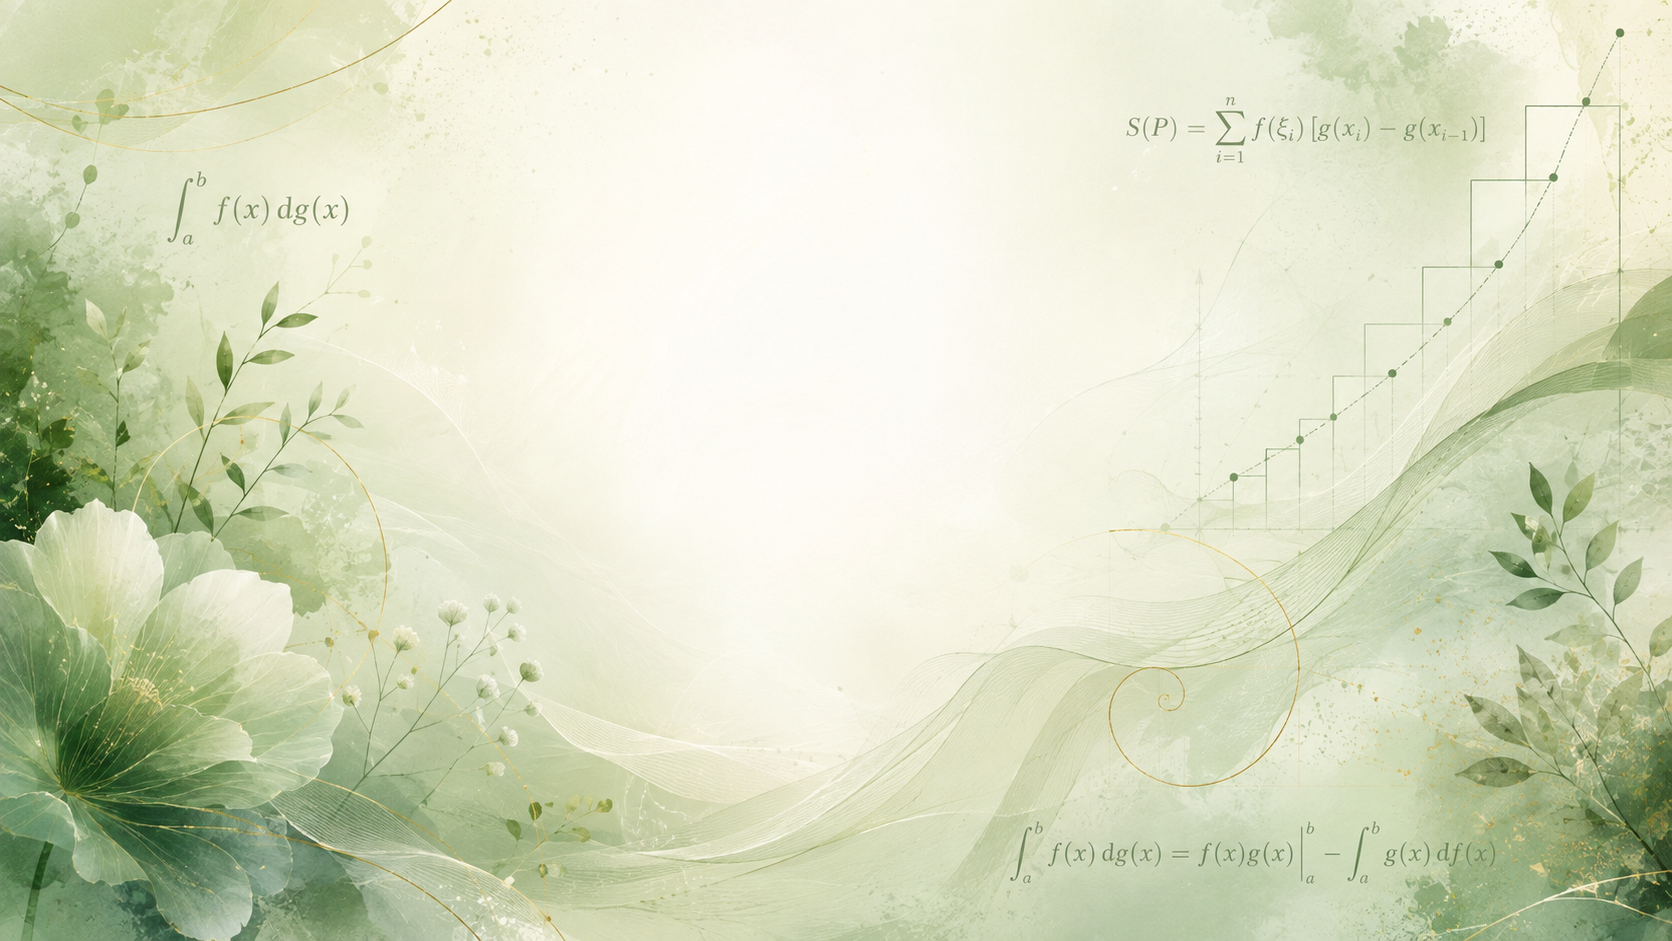
\includegraphics[width=\paperwidth,height=\paperheight,keepaspectratio=false]{chapter_06_bg_00.png}%
}
\begin{frame}[plain]
  \titlepage

  \note{
    Welcome to Chapter 6, Section 3: Integration and Differentiation.
    In the previous two episodes we built the Riemann-Stieltjes
    integral from scratch and developed its basic properties:
    linearity, order, products, and the reduction to the ordinary
    Riemann integral. In this episode we finally connect the two
    great operations of calculus. We will prove that integration and
    differentiation are, in a precise sense, inverse operations.
    The centerpiece is the Fundamental Theorem of Calculus, the
    result that lets us evaluate integrals by finding
    antiderivatives. Along the way we will see that integrating a
    function always produces something smoother than what we
    started with, and we will close with the integration by parts
    formula. Throughout this episode we work with the ordinary
    Riemann integral, and all functions are real valued. Let's begin.
  }
\end{frame}
}

{
\usebackgroundtemplate{%
  
\includegraphics[width=\paperwidth,height=\paperheight,keepaspectratio=false]{chapter_06_bg_01.png}%
}
\begin{frame}[c]{Outline}
  \begin{center}
    \tableofcontents
  \end{center}

  \note{
    Here is the plan. After a short motivation, we study the function
    you get by integrating "f" from "a" up to a variable endpoint
    "x". Theorem 6.20 says this new function is always continuous,
    and that it is differentiable with derivative "f" at every point
    where "f" is continuous. Then comes the star of the episode,
    Theorem 6.21, the Fundamental Theorem of Calculus: if "f" is
    integrable and has an antiderivative "F", then the integral of
    "f" over the whole interval is just "F" of "b" minus "F" of "a".
    The proof is a beautiful application of the mean value theorem
    from Chapter 5. Finally, Theorem 6.22 derives the integration by
    parts formula as a quick corollary, and we point out that it is
    the continuous twin of the summation by parts formula from
    Chapter 3. We finish with a summary and a preview of the next
    episode.
  }
\end{frame}

\section{Motivation}

% --- Build 1/3 ---
\begin{frame}{Two Operations, One Story}
  \begin{hlbox}
  \begin{itemize}
    \item Chapter 5: the \alert{derivative} --- a limit of difference
      quotients, measuring \emph{local} rate of change
    \item Chapter 6: the \alert{integral} --- a limit of sums,
      measuring \emph{global} accumulation
  \end{itemize}
  \end{hlbox}

  \note{
    So far, the two halves of calculus have lived separate lives. In
    Chapter 5 we studied the derivative, defined as a limit of
    difference quotients. It is a local object: it looks at a
    function through a microscope at a single point and reports the
    instantaneous rate of change. In this chapter we built the
    integral, defined through upper and lower sums over partitions.
    It is a global object: it adds up the values of a function
    across an entire interval. Next, the obvious question.
  }
\end{frame}

% --- Build 2/3 ---
\begin{frame}{Two Operations, One Story}
  \begin{hlbox}
  \begin{itemize}
    \item Chapter 5: the \alert{derivative} --- a limit of difference
      quotients, measuring \emph{local} rate of change
    \item Chapter 6: the \alert{integral} --- a limit of sums,
      measuring \emph{global} accumulation
    \item On the surface these constructions share \emph{nothing} ---
      yet they \alert{undo each other}
  \end{itemize}
  \end{hlbox}

  \note{
    Notice that nothing in the two definitions hints at a
    connection. One is built from quotients, the other from sums.
    And yet the great discovery of Newton and Leibniz, the discovery
    that turned calculus into a usable tool, is that these two
    operations undo each other. Differentiating an integral gives
    back the original function, and integrating a derivative
    recovers the original function up to its starting value. Our
    goal in this section is to state and prove this precisely.
  }
\end{frame}

% --- Build 3/3 ---
\begin{frame}{Two Operations, One Story}
  \begin{hlbox}
  \begin{itemize}
    \item Chapter 5: the \alert{derivative} --- a limit of difference
      quotients, measuring \emph{local} rate of change
    \item Chapter 6: the \alert{integral} --- a limit of sums,
      measuring \emph{global} accumulation
    \item On the surface these constructions share \emph{nothing} ---
      yet they \alert{undo each other}
    \item This section: real functions, ordinary Riemann integral
      ($\alpha(x) = x$)
  \end{itemize}
  \end{hlbox}

  \note{
    One remark on the setting before we start. In this section we
    still confine ourselves to real valued functions, and we work
    with the ordinary Riemann integral, that is, the Stieltjes
    integral with the weight alpha of "x" equal to "x". This is the
    setting where the derivative and the integral speak the same
    language. Let's preview the three results we are going to prove.
  }
\end{frame}

% --- Build 1/3 ---
\begin{frame}{What We Will Prove}
  \begin{hlbox}
  \begin{itemize}
    \item \textbf{Theorem 6.20:} differentiate the integral
      $F(x) = \int_a^x f(t)\,dt$ \\
      $\Rightarrow$ get $f$ back (where $f$ is continuous)
  \end{itemize}
  \end{hlbox}

  \note{
    Here is the roadmap. The first result, Theorem 6.20, goes from
    integration to differentiation. We fix the lower endpoint "a"
    and let the upper endpoint "x" vary, obtaining a new function
    "F" of "x", the integral of "f" from "a" to "x". The theorem
    says that "F" is always continuous, and that at every point
    where "f" itself is continuous, "F" is differentiable with
    derivative exactly "f". Differentiating the integral recovers
    the function.
  }
\end{frame}

% --- Build 2/3 ---
\begin{frame}{What We Will Prove}
  \begin{hlbox}
  \begin{itemize}
    \item \textbf{Theorem 6.20:} differentiate the integral
      $F(x) = \int_a^x f(t)\,dt$ \\
      $\Rightarrow$ get $f$ back (where $f$ is continuous)
    \item \textbf{Theorem 6.21 (FTC):} integrate the derivative
      $F' = f$ \\
      $\Rightarrow$ get $\int_a^b f(x)\,dx = F(b) - F(a)$
  \end{itemize}
  \end{hlbox}

  \note{
    The second result goes the other way, from differentiation to
    integration. This is the Fundamental Theorem of Calculus,
    Theorem 6.21. If "f" is integrable and we can find any
    differentiable function "F" whose derivative is "f", then the
    integral of "f" over the interval equals "F" of "b" minus "F"
    of "a". This is the theorem you have used every time you
    evaluated an integral by finding an antiderivative. Now we get
    to see exactly why it is true, and under exactly what
    hypotheses.
  }
\end{frame}

% --- Build 3/3 ---
\begin{frame}{What We Will Prove}
  \begin{hlbox}
  \begin{itemize}
    \item \textbf{Theorem 6.20:} differentiate the integral
      $F(x) = \int_a^x f(t)\,dt$ \\
      $\Rightarrow$ get $f$ back (where $f$ is continuous)
    \item \textbf{Theorem 6.21 (FTC):} integrate the derivative
      $F' = f$ \\
      $\Rightarrow$ get $\int_a^b f(x)\,dx = F(b) - F(a)$
    \item \textbf{Theorem 6.22:} \alert{integration by parts} ---
      the product rule, run backwards through the FTC
  \end{itemize}
  \end{hlbox}

  \note{
    And once the Fundamental Theorem is in hand, useful corollaries
    follow almost for free. Theorem 6.22 is the integration by parts
    formula: it is nothing more than the product rule for
    derivatives, fed through the Fundamental Theorem. It converts
    one integral into another, often simpler one, and it will be a
    workhorse in later chapters, for example in the theory of
    Fourier series. Let's start with Theorem 6.20 and the idea of
    integrating up to a variable endpoint.
  }
\end{frame}

}

{
\usebackgroundtemplate{%
  
\includegraphics[width=\paperwidth,height=\paperheight,keepaspectratio=false]{chapter_06_bg_02.png}%
}
\section{The Integral as a Function of Its Upper Limit}

\begin{frame}{A New Function: The Area So Far}
  \begin{hlbox}
  For $f \in \mathscr{R}$ on $[a, b]$ and $a \leq x \leq b$, define
  \[
    F(x) = \int_a^x f(t)\,dt.
  \]
  \end{hlbox}

  \begin{center}
  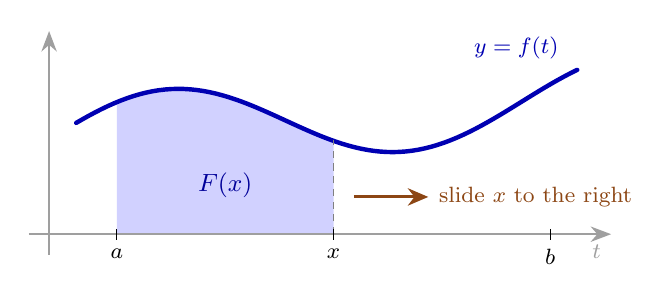
\begin{tikzpicture}[scale=0.86]
    % shaded region a..x under curve (drawn first so axes stay visible)
    \begin{scope}
      \clip (1.0,0) rectangle (4.2,3.0);
      \fill[blue!18] plot[domain=0.4:7.8, samples=80]
        (\x, {1.4 + 0.6*sin(deg(0.9*\x)) + 0.08*\x}) -- (7.8,0) -- (0.4,0) -- cycle;
    \end{scope}
    \draw[axisln] (-0.3,0) -- (8.3,0) node[below left]{\footnotesize $t$};
    \draw[axisln] (0,-0.3) -- (0,3.0);
    % curve f
    \draw[curveln, blue!70!black, domain=0.4:7.8, samples=80]
      plot (\x, {1.4 + 0.6*sin(deg(0.9*\x)) + 0.08*\x});
    \draw[projln, gray] (4.2,0) -- (4.2,1.39);
    \node[blue!60!black] at (2.6, 0.72) {\small $F(x)$};
    \draw (1.0,0.08) -- (1.0,-0.08) node[below]{\footnotesize $a$};
    \draw (4.2,0.08) -- (4.2,-0.08) node[below]{\footnotesize $x$};
    \draw (7.4,0.08) -- (7.4,-0.08) node[below]{\footnotesize $b$};
    \node[blue!70!black] at (6.9, 2.75) {\footnotesize $y = f(t)$};
    \draw[guide, mAccent] (4.5,0.55) -- (5.6,0.55)
      node[right]{\footnotesize slide $x$ to the right};
  \end{tikzpicture}
  \end{center}

  \note{
    Here is the central object of this section. Take an integrable
    function "f" on the interval from "a" to "b". Instead of
    integrating all the way to "b", we stop at a variable point "x",
    and we call the result "F" of "x". In the picture, the blue
    curve is the graph of "f", and the shaded blue region is the
    area accumulated between "a" and the dashed line at "x". As the
    orange arrow suggests, when "x" slides to the right, the shaded
    region grows, so "F" is a function of "x": the area so far. The
    natural question is how smooth this new function is, and that is
    exactly what Theorem 6.20 answers.
  }
\end{frame}

% --- Build 1/2 ---
\begin{frame}{Theorem 6.20: Differentiating the Integral}
  \begin{thmblock}{Theorem 6.20}
    Let $f \in \mathscr{R}$ on $[a, b]$. For $a \leq x \leq b$, put
    \[
      F(x) = \int_a^x f(t)\,dt.
    \]
    Then $F$ is \alert{continuous} on $[a, b]$.
  \end{thmblock}

  \note{
    Theorem 6.20 has two conclusions, and we take them one at a
    time. The first is unconditional: whenever "f" is integrable,
    the accumulated area function "F" is continuous on the whole
    interval, in fact uniformly continuous, as the proof will show.
    Think about what this says: "f" itself may jump around, it only
    needs to be integrable, but the process of integration smooths
    it out into a continuous function. Integration is a smoothing
    operation. And if "f" is even a little better than integrable,
    we get more.
  }
\end{frame}

% --- Build 2/2 ---
\begin{frame}{Theorem 6.20: Differentiating the Integral}
  \begin{thmblock}{Theorem 6.20}
    Let $f \in \mathscr{R}$ on $[a, b]$. For $a \leq x \leq b$, put
    \[
      F(x) = \int_a^x f(t)\,dt.
    \]
    Then $F$ is \alert{continuous} on $[a, b]$; furthermore, if $f$ is
    continuous at a point $x_0$ of $[a, b]$, then $F$ is
    \alert{differentiable} at $x_0$, and
    \[
      F'(x_0) = f(x_0).
    \]
  \end{thmblock}

  \note{
    The second conclusion is the inverse relationship. At any point
    "x" sub 0 where "f" happens to be continuous, the function "F"
    is differentiable there, and its derivative is exactly the value
    "f" of "x" sub 0. So each degree of regularity of "f" is
    upgraded by one: integrable becomes continuous, and continuous
    becomes differentiable. In particular, if "f" is continuous on
    the whole interval, then "F" is an antiderivative of "f", so
    every continuous function has an antiderivative. Before proving
    this, let's look at an example that shows why continuity of "f"
    at the point really matters.
  }
\end{frame}

\begin{frame}{Example: A Jump Becomes a Corner}
  \begin{exblock}{Integrating a step}
    On $[-1, 1]$, let $f(t) = 0$ for $t < 0$ and $f(t) = 1$ for
    $t \geq 0$. Then
    $F(x) = \int_{-1}^x f(t)\,dt = \max(x, 0)$.
  \end{exblock}

  \begin{center}
  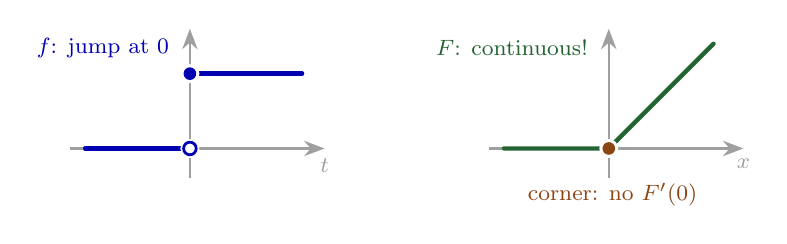
\begin{tikzpicture}[scale=0.95]
    % left: f
    \begin{scope}
      \draw[axisln] (-1.6,0) -- (1.8,0) node[below]{\footnotesize $t$};
      \draw[axisln] (0,-0.4) -- (0,1.6);
      \draw[curveln, blue!70!black] (-1.4,0) -- (0,0);
      \draw[curveln, blue!70!black] (0,1) -- (1.5,1);
      \opendotpt{blue!70!black}{(0,0)}
      \dotpt{blue!70!black}{(0,1)}
      \node[blue!70!black, anchor=east] at (-0.15,1.35)
        {\footnotesize $f$: jump at $0$};
    \end{scope}
    % right: F
    \begin{scope}[xshift=5.6cm]
      \draw[axisln] (-1.6,0) -- (1.8,0) node[below]{\footnotesize $x$};
      \draw[axisln] (0,-0.4) -- (0,1.6);
      \draw[curveln, proofcolor] (-1.4,0) -- (0,0) -- (1.4,1.4);
      \dotpt{mAccent}{(0,0)}
      \node[mAccent] at (0.05,-0.62) {\footnotesize corner: no $F'(0)$};
      \node[proofcolor, anchor=east] at (-0.15,1.35)
        {\footnotesize $F$: continuous!};
    \end{scope}
  \end{tikzpicture}
  \end{center}

  \note{
    Let's test the theorem on the simplest discontinuous function.
    On the left, "f" is a step: zero for negative "t", one for
    nonnegative "t", with a jump at zero. Integrating from minus one
    up to "x" gives the function on the right: "F" of "x" is zero
    while "x" is negative, and then grows like "x" afterwards. Just
    as the theorem promised, "F" is continuous everywhere, the jump
    has been smoothed into an unbroken graph. But look at the orange
    point: at zero, exactly where "f" jumps, the graph of "F" has a
    corner. The slope from the left is zero and the slope from the
    right is one, so "F" is not differentiable there. Away from
    zero, where "f" is continuous, the derivative of "F" equals "f"
    exactly. The theorem is sharp. Now let's see the proof strategy.
  }
\end{frame}

\begin{frame}{Proof Strategy: Theorem 6.20}
  \begin{hlbox}
  \textbf{Two parts, two tools:}
  \begin{enumerate}
    \item \textbf{Continuity of $F$:} the size bound of Theorem
      6.12($c$),($d$) gives
      $|F(y) - F(x)| \leq M(y - x)$
    \item \textbf{Differentiability at $x_0$:} the difference quotient
      of $F$ is an \alert{average} of $f$, and averages of $f$ near
      $x_0$ are close to $f(x_0)$
  \end{enumerate}
  \end{hlbox}

  \vspace{0.5em}
  \begin{remblock}{Recall: Theorem 6.12($c$), ($d$)}
    The integral splits at any intermediate point, and
    $\bigl|\int f\,dx\bigr| \leq M \cdot (\text{length of the interval})$
    when $|f| \leq M$.
  \end{remblock}

  \note{
    The proof has two parts, matching the two conclusions. For
    continuity, the only tool we need is the basic size bound from
    the last episode. As the recall box says, the integral over an
    interval is at most the bound on the function times the length
    of the interval; combined with the splitting property, the
    difference of "F" at two points is the integral over the short
    interval between them, hence small. For differentiability, the
    key observation is that the difference quotient of "F" is not
    just related to "f", it is precisely the average value of "f"
    over a small interval. If "f" is continuous at "x" sub 0, then
    near "x" sub 0 the function stays close to "f" of "x" sub 0, so
    its averages do too. Let's carry this out.
  }
\end{frame}

% --- Build 1/2 ---
\begin{frame}{Proof of Theorem 6.20 --- Part 1: Continuity}
  \begin{columns}[T]
    \begin{column}{0.58\textwidth}
      \begin{proofblock}{Step 1: A Lipschitz bound}
        $f \in \mathscr{R}$ is bounded: say $|f(t)| \leq M$.
        For $a \leq x < y \leq b$,
        \[
          |F(y) - F(x)| = \left|\int_x^y f(t)\,dt\right| \leq M(y - x)
        \]
        by Theorem 6.12($c$) and ($d$).
      \end{proofblock}
    \end{column}
    \begin{column}{0.40\textwidth}
      \vspace{0.4em}
      \begin{center}
      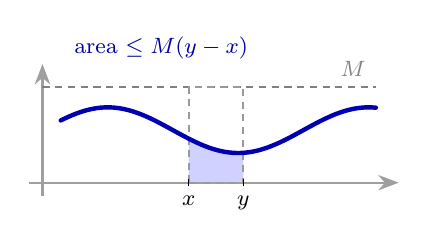
\begin{tikzpicture}[scale=0.58]
        % area under the curve on [x,y] (drawn first so axes stay visible)
        \begin{scope}
          \clip (3.2,0) rectangle (4.4,2.6);
          \fill[blue!18] plot[domain=0.4:7.3, samples=80]
            (\x, {1.15 + 0.5*sin(deg(1.1*\x))}) -- (7.3,0) -- (0.4,0) -- cycle;
        \end{scope}
        \draw[axisln] (-0.3,0) -- (7.8,0);
        \draw[axisln] (0,-0.3) -- (0,2.6);
        \draw[projln, gray] (0,2.1) -- (7.3,2.1)
          node[above left]{\footnotesize $M$};
        % the M-height rectangle enclosing that area
        \draw[projln, gray!80] (3.2,0) rectangle (4.4,2.1);
        \draw[curveln, blue!70!black, domain=0.4:7.3, samples=80]
          plot (\x, {1.15 + 0.5*sin(deg(1.1*\x))});
        \draw (3.2,0.08) -- (3.2,-0.08) node[below]{\footnotesize $x$};
        \draw (4.4,0.08) -- (4.4,-0.08) node[below]{\footnotesize $y$};
        \node[blue!60!black] at (2.6,2.95)
          {\footnotesize area $\leq M(y-x)$};
      \end{tikzpicture}
      \end{center}
    \end{column}
  \end{columns}

  \note{
    Here is part 1. Since "f" is integrable, it is bounded, so pick
    "M" with the absolute value of "f" at most "M" everywhere. Now
    take two points "x" less than "y". By the splitting property,
    "F" of "y" minus "F" of "x" is just the integral of "f" over the
    short interval from "x" to "y", and by the size bound, its
    absolute value is at most "M" times "y" minus "x". The picture
    shows why: the shaded area under the curve between "x" and "y"
    fits inside the dashed rectangle of height "M", so the
    accumulated area cannot change
    faster than "M" times the width. The change in "F" is controlled
    linearly by the change in "x". Next, we turn this into
    continuity.
  }
\end{frame}

% --- Build 2/2 ---
\begin{frame}{Proof of Theorem 6.20 --- Part 1: Continuity}
  \begin{columns}[T]
    \begin{column}{0.58\textwidth}
      \begin{proofblock}{Step 1: A Lipschitz bound}
        $f \in \mathscr{R}$ is bounded: say $|f(t)| \leq M$.
        For $a \leq x < y \leq b$,
        \[
          |F(y) - F(x)| = \left|\int_x^y f(t)\,dt\right| \leq M(y - x)
        \]
        by Theorem 6.12($c$) and ($d$).
      \end{proofblock}
    \end{column}
    \begin{column}{0.40\textwidth}
      \vspace{0.4em}
      \begin{center}
      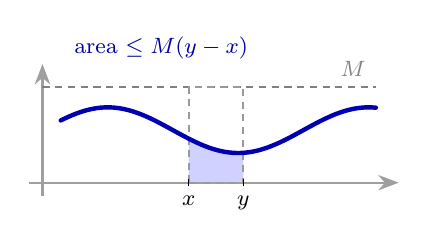
\begin{tikzpicture}[scale=0.58]
        % area under the curve on [x,y] (drawn first so axes stay visible)
        \begin{scope}
          \clip (3.2,0) rectangle (4.4,2.6);
          \fill[blue!18] plot[domain=0.4:7.3, samples=80]
            (\x, {1.15 + 0.5*sin(deg(1.1*\x))}) -- (7.3,0) -- (0.4,0) -- cycle;
        \end{scope}
        \draw[axisln] (-0.3,0) -- (7.8,0);
        \draw[axisln] (0,-0.3) -- (0,2.6);
        \draw[projln, gray] (0,2.1) -- (7.3,2.1)
          node[above left]{\footnotesize $M$};
        % the M-height rectangle enclosing that area
        \draw[projln, gray!80] (3.2,0) rectangle (4.4,2.1);
        \draw[curveln, blue!70!black, domain=0.4:7.3, samples=80]
          plot (\x, {1.15 + 0.5*sin(deg(1.1*\x))});
        \draw (3.2,0.08) -- (3.2,-0.08) node[below]{\footnotesize $x$};
        \draw (4.4,0.08) -- (4.4,-0.08) node[below]{\footnotesize $y$};
        \node[blue!60!black] at (2.6,2.95)
          {\footnotesize area $\leq M(y-x)$};
      \end{tikzpicture}
      \end{center}
    \end{column}
  \end{columns}

  \begin{proofblock}{Step 2: Uniform continuity}
    $|y - x| < \varepsilon/M \implies |F(y) - F(x)| < \varepsilon$.
    \quad $\boxed{F \text{ is uniformly continuous.}}$
  \end{proofblock}

  \note{
    Step 2 is immediate. Given any positive epsilon, choose delta to
    be epsilon over "M". Whenever two points are within delta of
    each other, the bound from step 1 makes the values of "F"
    within epsilon of each other. Notice that this delta depends
    only on epsilon and "M", not on the location of the points, so
    we have proved uniform continuity, which is stronger than what
    the theorem asked for. Part 1 is complete: integrating any
    integrable function produces a continuous, indeed Lipschitz,
    function. Now for the more interesting part: differentiability
    at points where "f" is continuous.
  }
\end{frame}

% --- Build 1/3 ---
\begin{frame}{Proof of Theorem 6.20 --- Part 2: Differentiability}
  \begin{proofblock}{Step 1: Use continuity of $f$ at $x_0$}
    Given $\varepsilon > 0$, choose $\delta > 0$ so that
    $|f(u) - f(x_0)| < \varepsilon$ whenever
    $|u - x_0| < \delta$ and $u \in [a,b]$.
  \end{proofblock}

  \note{
    Suppose now that "f" is continuous at the point "x" sub 0. We
    want to show the difference quotient of "F" converges to "f" of
    "x" sub 0. Let epsilon be given. Continuity of "f" at "x" sub 0
    hands us a delta: every point "u" within delta of "x" sub 0 has
    its value "f" of "u" within epsilon of "f" of "x" sub 0. In
    other words, on this small window around "x" sub 0, the whole
    graph of "f" lives in a band of height epsilon around the value
    "f" of "x" sub 0. That band is the only fact we will use. Next
    comes the key computation.
  }
\end{frame}

% --- Build 2/3 ---
\begin{frame}{Proof of Theorem 6.20 --- Part 2: Differentiability}
  \begin{proofblock}{Step 1: Use continuity of $f$ at $x_0$}
    Given $\varepsilon > 0$, choose $\delta > 0$ so that
    $|f(u) - f(x_0)| < \varepsilon$ whenever
    $|u - x_0| < \delta$ and $u \in [a,b]$.
  \end{proofblock}

  \begin{proofblock}{Step 2: The difference quotient is an average}
    For $x_0 - \delta < s \leq x_0 \leq t < x_0 + \delta$ (inside
    $[a,b]$), Theorem 6.12($d$) gives:
    \[
      \left|\frac{F(t) - F(s)}{t - s} - f(x_0)\right|
      = \left|\frac{1}{t-s}\int_s^t [f(u) - f(x_0)]\,du\right|
      < \varepsilon.
    \]
  \end{proofblock}

  \note{
    Step 2 is the heart of the proof. Take any two points "s" and
    "t" inside the delta window, with "s" on the left of "x" sub 0
    and "t" on the right. Look at the identity on the slide. The
    difference quotient, "F" of "t" minus "F" of "s" over "t" minus
    "s", is exactly the average value of "f" on the interval from
    "s" to "t". So subtracting "f" of "x" sub 0 gives the average of
    the difference "f" of "u" minus "f" of "x" sub 0. But step 1
    says that difference is smaller than epsilon everywhere in the
    window, and the average of numbers smaller than epsilon is
    smaller than epsilon, by the size bound of Theorem 6.12. The
    average of "f" over a tiny window hugs "f" of "x" sub 0.
  }
\end{frame}

% --- Build 3/3 ---
\begin{frame}{Proof of Theorem 6.20 --- Part 2: Differentiability}
  \begin{proofblock}{Step 1: Use continuity of $f$ at $x_0$}
    Given $\varepsilon > 0$, choose $\delta > 0$ so that
    $|f(u) - f(x_0)| < \varepsilon$ whenever
    $|u - x_0| < \delta$ and $u \in [a,b]$.
  \end{proofblock}

  \begin{proofblock}{Step 2: The difference quotient is an average}
    For $x_0 - \delta < s \leq x_0 \leq t < x_0 + \delta$ (inside
    $[a,b]$), Theorem 6.12($d$) gives:
    \[
      \left|\frac{F(t) - F(s)}{t - s} - f(x_0)\right|
      = \left|\frac{1}{t-s}\int_s^t [f(u) - f(x_0)]\,du\right|
      < \varepsilon.
    \]
  \end{proofblock}

  \vspace{-0.3em}
  \hl{\textbf{Conclusion:} letting $s, t \to x_0$: \
    $\boxed{F'(x_0) = f(x_0).}$ \ $\blacksquare$}

  \note{
    And now we are done. The estimate in step 2 holds for every pair
    "s", "t" straddling "x" sub 0 inside the delta window, and
    epsilon was arbitrary. Taking "s" and "t" to approach "x" sub 0,
    in particular taking one of them equal to "x" sub 0 itself, the
    difference quotients of "F" converge to "f" of "x" sub 0. So
    "F" prime of "x" sub 0 exists and equals "f" of "x" sub 0,
    which completes the proof of Theorem 6.20. Differentiating the
    accumulated area recovers the integrand at every point of
    continuity. With this in hand, we are ready for the main event:
    the Fundamental Theorem of Calculus.
  }
\end{frame}

}

{
\usebackgroundtemplate{%
  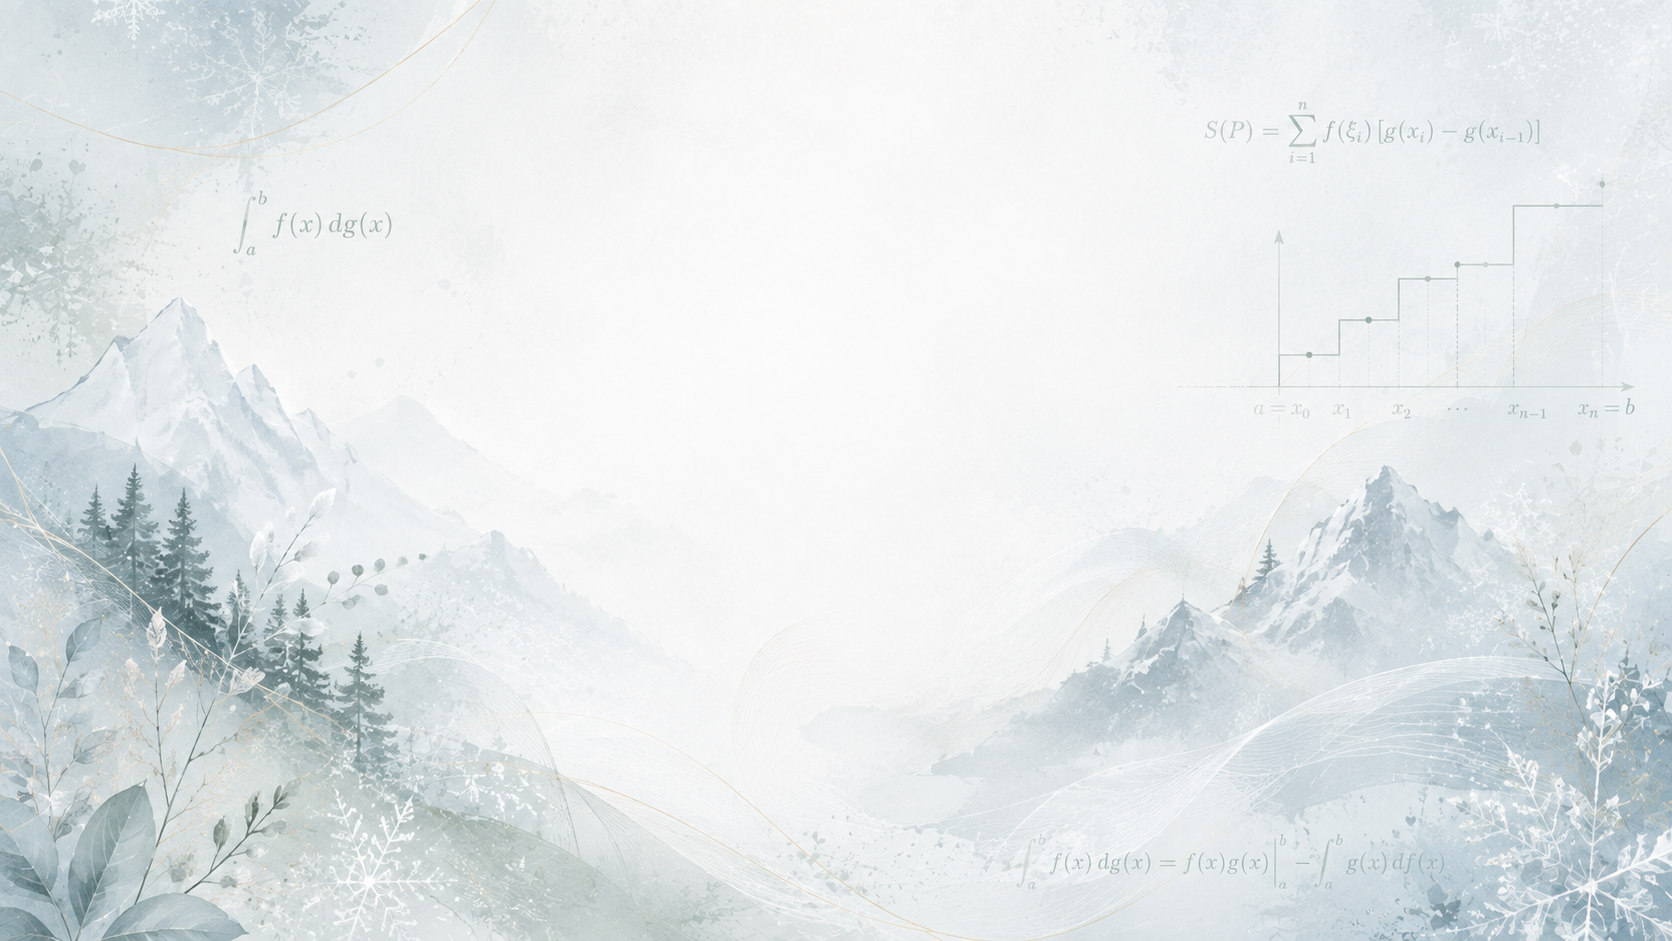
\includegraphics[width=\paperwidth,height=\paperheight,keepaspectratio=false]{chapter_06_bg_03.png}%
}
\section{The Fundamental Theorem of Calculus}

\begin{frame}{Theorem 6.21: The Fundamental Theorem of Calculus}
  \begin{thmblock}{Theorem 6.21 (Fundamental Theorem of Calculus)}
    If $f \in \mathscr{R}$ on $[a, b]$ and if there is a
    differentiable function $F$ on $[a, b]$ such that $F' = f$, then
    \[
      \int_a^b f(x)\,dx = F(b) - F(a).
    \]
  \end{thmblock}

  \vspace{0.6em}
  \begin{hlbox}
    \textbf{In words:} to integrate $f$, find \emph{any}
    antiderivative $F$ and take the \alert{net change} $F(b) - F(a)$.
  \end{hlbox}

  \note{
    Here it is: the Fundamental Theorem of Calculus, Theorem 6.21.
    The hypotheses are two: first, "f" must be Riemann integrable on
    the interval, and second, "f" must have an antiderivative, a
    differentiable function "F" whose derivative is "f" at every
    point of the interval. The conclusion is the formula you know:
    the integral of "f" from "a" to "b" equals "F" of "b" minus "F"
    of "a". In words, a limit of complicated Riemann sums collapses
    to a single subtraction, the net change of the antiderivative.
    This is what makes integrals computable in practice: instead of
    wrestling with partitions and suprema, you hunt for an
    antiderivative and evaluate it at the two endpoints. Before the
    proof, one remark about the hypotheses.
  }
\end{frame}

\begin{frame}{Remark: Reading the Hypotheses Carefully}
  \begin{remblock}{Both hypotheses are needed}
    \begin{itemize}
      \item $f$ need \emph{not} be continuous --- integrability
        suffices. But integrability must be \emph{assumed}: a
        derivative $F'$ can fail to be in $\mathscr{R}$.
      \item If $f$ \emph{is} continuous on $[a,b]$, Theorem 6.20
        provides an antiderivative automatically --- both hypotheses
        hold for free.
    \end{itemize}
  \end{remblock}

  \note{
    Two comments on the hypotheses. First, notice how little is
    asked of "f": no continuity, just integrability plus the
    existence of an antiderivative. That makes this statement more
    general than the version usually taught in a first calculus
    course. But the integrability assumption cannot be dropped:
    there exist differentiable functions "F" whose derivative is so
    wild that it fails to be Riemann integrable, and then the left
    hand side of the formula does not even make sense. Second, the
    two theorems of this episode work together beautifully. If "f"
    is continuous on the whole interval, then Theorem 6.20 already
    manufactures an antiderivative for us, namely the accumulated
    area function, and "f" is integrable by Theorem 6.8. So for
    continuous functions, the Fundamental Theorem applies with no
    further checking. Now, the proof strategy.
  }
\end{frame}

\begin{frame}{Proof Strategy: Theorem 6.21}
  \hl{\textbf{Goal:} $\int_a^b f\,dx = F(b) - F(a)$.}

  \vspace{0.4em}
  \begin{hlbox}
  \textbf{Approach:}
  \begin{enumerate}
    \item Pick a partition $P$ with $U(P,f) - L(P,f) < \varepsilon$
      \hfill (Theorem 6.6)
    \item Apply the \alert{mean value theorem} on each subinterval:
      the change of $F$ across $[x_{i-1},x_i]$ is $f(t_i)\,\Delta x_i$
    \item Sum: the changes \alert{telescope} to $F(b) - F(a)$:
      \emph{exact} Riemann sum!
    \item Compare this sum with the integral \hfill (Theorem 6.7($c$))
  \end{enumerate}
  \end{hlbox}

  \note{
    Here is the plan of attack, in four steps. Step 1: since "f" is
    integrable, the Cauchy criterion of Theorem 6.6 lets us pick a
    partition whose upper and lower sums differ by less than
    epsilon. Step 2 is the masterstroke: on each subinterval of that
    partition, we apply the mean value theorem from Chapter 5 to
    "F". It tells us that the change of "F" across the subinterval
    is the value of "f" at some interior point times the length of
    the subinterval. Step 3: when we add these changes over all
    subintervals, the left hand sides telescope, leaving exactly "F"
    of "b" minus "F" of "a". So this particular Riemann sum does not
    just approximate the net change, it equals it exactly. Step 4:
    by Theorem 6.7 part "c", any Riemann sum built from a fine
    partition lies within epsilon of the integral. Let's look at the
    key picture first.
  }
\end{frame}

\begin{frame}{The Key Picture: MVT on Each Subinterval}
  \begin{center}
  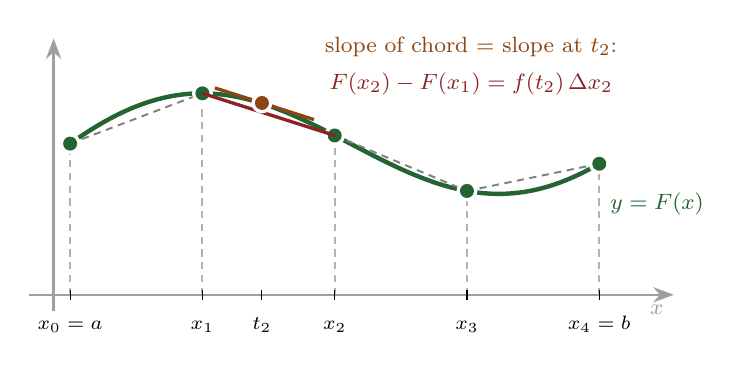
\begin{tikzpicture}[scale=1.05]
    \draw[axisln] (0.3,0) -- (8.1,0) node[below left]{\footnotesize $x$};
    \draw[axisln] (0.6,-0.2) -- (0.6,3.1);
    % curve F
    \draw[curveln, proofcolor, domain=0.8:7.2, samples=80]
      plot (\x, {1.2 + 0.15*\x + 0.9*sin(deg(0.75*\x))});
    \node[proofcolor] at (7.9,1.1) {\footnotesize $y = F(x)$};
    % partition points and chords
    \foreach \a/\b in {0.8/2.4, 2.4/4.0, 4.0/5.6, 5.6/7.2}{
      \draw[projln, gray]
        (\a, {1.2 + 0.15*\a + 0.9*sin(deg(0.75*\a))}) --
        (\b, {1.2 + 0.15*\b + 0.9*sin(deg(0.75*\b))});
    }
    \foreach \p/\lab in {0.8/{x_0 = a}, 2.4/{x_1}, 4.0/{x_2}, 5.6/{x_3}, 7.2/{x_4 = b}}{
      \draw[projln, gray!60] (\p,0) --
        (\p, {1.2 + 0.15*\p + 0.9*sin(deg(0.75*\p))});
      \draw (\p,0.06) -- (\p,-0.06);
      \node[anchor=base] at (\p,-0.42) {\scriptsize $\lab$};
      \dotpt{proofcolor}{(\p, {1.2 + 0.15*\p + 0.9*sin(deg(0.75*\p))})}
    }
    % highlighted subinterval [2.4, 4.0]: chord + parallel tangent at t=3.12
    \draw[thmcolor, line width=1.2pt]
      (2.4, {1.2 + 0.15*2.4 + 0.9*sin(deg(0.75*2.4))}) --
      (4.0, {1.2 + 0.15*4.0 + 0.9*sin(deg(0.75*4.0))});
    \draw[mAccent, line width=1.2pt] (2.55, 2.502) -- (3.75, 2.119);
    \dotpt{mAccent}{(3.12, 2.320)}
    \draw (3.12,0.06) -- (3.12,-0.06);
    \node[anchor=base] at (3.12,-0.42) {\scriptsize $t_2$};
    \node[mAccent, align=left] at (5.65,3.0)
      {\footnotesize slope of chord $=$ slope at $t_2$:};
    \node[thmcolor] at (5.65,2.55)
      {\footnotesize $F(x_2) - F(x_1) = f(t_2)\,\Delta x_2$};
  \end{tikzpicture}
  \end{center}

  \note{
    This picture carries the whole proof. The green curve is the
    graph of the antiderivative "F", and the points "x" sub 0
    through "x" sub 4 on the axis form our partition, with the green
    dots marking the corresponding points on the curve. The gray
    dashed segments are the chords over each subinterval. Focus on
    the highlighted subinterval from "x" sub 1 to "x" sub 2. The red
    segment is its chord, and its slope is the change of "F" divided
    by the width. The mean value theorem says that somewhere inside,
    at a point we call "t" sub 2, the tangent to the curve, drawn in
    orange, is parallel to that chord. Since the slope of the
    tangent is "F" prime, which is "f", we get the identity on the
    slide: the change of "F" across the subinterval equals "f" of
    "t" sub 2 times delta "x" sub 2. The same happens in every
    subinterval, and this is the bridge between "F" and the Riemann
    sums of "f". Let's now write the proof.
  }
\end{frame}

% --- Build 1/4 ---
\begin{frame}{Proof of Theorem 6.21}
  \begin{proofblock}{Step 1: A fine partition}
    Let $\varepsilon > 0$. Since $f \in \mathscr{R}$, Theorem 6.6
    gives a partition $P = \{x_0, \dots, x_n\}$ with
    $U(P, f) - L(P, f) < \varepsilon$.
  \end{proofblock}

  \note{
    The formal proof now takes four short steps. Step 1: let epsilon
    be given. Because "f" is Riemann integrable, the criterion of
    Theorem 6.6 from two episodes ago applies: we can choose a
    partition "P", with points "x" sub 0 up to "x" sub "n", so fine
    that its upper sum and lower sum differ by less than epsilon.
    Everything that follows happens on this one partition. Next, the
    mean value theorem enters.
  }
\end{frame}

% --- Build 2/4 ---
\begin{frame}{Proof of Theorem 6.21}
  \begin{proofblock}{Step 1: A fine partition}
    Let $\varepsilon > 0$. Since $f \in \mathscr{R}$, Theorem 6.6
    gives a partition $P = \{x_0, \dots, x_n\}$ with
    $U(P, f) - L(P, f) < \varepsilon$.
  \end{proofblock}

  \begin{proofblock}{Step 2: Mean value theorem on each subinterval}
    Since $F' = f$, the MVT (Theorem 5.10) furnishes points
    $t_i \in [x_{i-1}, x_i]$, $i = 1, \dots, n$, with \
    $F(x_i) - F(x_{i-1}) = f(t_i)\,\Delta x_i$.
  \end{proofblock}

  \note{
    Step 2: on each subinterval from "x" sub "i" minus 1 to "x" sub
    "i", the function "F" is differentiable, so the mean value
    theorem, Theorem 5.10 from Chapter 5, applies. It furnishes a
    point "t" sub "i" inside the subinterval where the derivative of
    "F" equals the slope of the chord. But the derivative of "F" is
    "f". So the change of "F" across the subinterval is exactly "f"
    of "t" sub "i" times delta "x" sub "i", just as we saw in the
    picture. Note that we do not get to choose the points "t" sub
    "i"; the mean value theorem chooses them for us. The miracle is
    that we do not need any control over where they are. Now we add
    everything up.
  }
\end{frame}

% --- Build 3/4 ---
\begin{frame}{Proof of Theorem 6.21}
  \begin{proofblock}{Step 1: A fine partition}
    Let $\varepsilon > 0$. Since $f \in \mathscr{R}$, Theorem 6.6
    gives a partition $P = \{x_0, \dots, x_n\}$ with
    $U(P, f) - L(P, f) < \varepsilon$.
  \end{proofblock}

  \begin{proofblock}{Step 2: Mean value theorem on each subinterval}
    Since $F' = f$, the MVT (Theorem 5.10) furnishes points
    $t_i \in [x_{i-1}, x_i]$, $i = 1, \dots, n$, with \
    $F(x_i) - F(x_{i-1}) = f(t_i)\,\Delta x_i$.
  \end{proofblock}

  \begin{proofblock}{Step 3: The sum telescopes}
    \[
      \textstyle\sum_{i=1}^{n} f(t_i)\,\Delta x_i
      = \sum_{i=1}^{n} \bigl[F(x_i) - F(x_{i-1})\bigr]
      = \boxed{F(b) - F(a).}
    \]
  \end{proofblock}

  \note{
    Step 3: sum the identity of step 2 over all subintervals. On the
    left we get the Riemann sum of "f" with the sample points "t"
    sub "i". On the right we get a telescoping sum: "F" of "x" sub 1
    minus "F" of "x" sub 0, plus "F" of "x" sub 2 minus "F" of "x"
    sub 1, and so on. Every intermediate value cancels with its
    neighbor, leaving only "F" of the last point minus "F" of the
    first, that is, "F" of "b" minus "F" of "a". So this particular
    Riemann sum equals the net change of "F" exactly, not just
    approximately. One step remains: relate this sum to the
    integral.
  }
\end{frame}

% --- Build 4/4 ---
\begin{frame}{Proof of Theorem 6.21}
  \begin{proofblock}{Steps 1--3 (summary)}
    $U(P,f) - L(P,f) < \varepsilon$, \quad and the MVT gives
    $\sum_{i=1}^{n} f(t_i)\,\Delta x_i = F(b) - F(a)$.
  \end{proofblock}

  \begin{proofblock}{Step 4: Compare with the integral}
    Theorem 6.7($c$): \emph{every} Riemann sum on such a $P$ is
    within $\varepsilon$ of the integral:
    \[
      \Bigl|F(b) - F(a) - \int_a^b f(x)\,dx\Bigr| < \varepsilon.
    \]
    True for \emph{every} $\varepsilon > 0$, so \
    $\boxed{\int_a^b f(x)\,dx = F(b) - F(a).}$ \hfill $\blacksquare$
  \end{proofblock}

  \note{
    Step 4 closes the loop. Recall Theorem 6.7 part "c" from two
    episodes ago: for a partition whose upper and lower sums are
    within epsilon, every Riemann sum, no matter which sample points
    are used, lies within epsilon of the integral. Our sample points
    "t" sub "i" came from the mean value theorem, but the theorem
    does not care; arbitrary means arbitrary. So "F" of "b" minus
    "F" of "a", which equals our Riemann sum, differs from the
    integral by less than epsilon. And since epsilon was an
    arbitrary positive number, the difference must be zero. The
    integral of "f" equals "F" of "b" minus "F" of "a", and the
    Fundamental Theorem of Calculus is proved. Notice how short the
    argument was: all the heavy lifting was done by the mean value
    theorem and the integration theory we already built. Next, a
    classic corollary.
  }
\end{frame}

}

{
\usebackgroundtemplate{%
  
\includegraphics[width=\paperwidth,height=\paperheight,keepaspectratio=false]{chapter_06_bg_04.png}%
}
\section{Integration by Parts}

\begin{frame}{Theorem 6.22: Integration by Parts}
  \begin{thmblock}{Theorem 6.22 (integration by parts)}
    Suppose $F$ and $G$ are differentiable functions on $[a, b]$,
    $F' = f \in \mathscr{R}$, and $G' = g \in \mathscr{R}$. Then
    \[
      \int_a^b F(x)g(x)\,dx
      = F(b)G(b) - F(a)G(a) - \int_a^b f(x)G(x)\,dx.
    \]
  \end{thmblock}

  \vspace{0.6em}
  \hl{\textbf{Key idea:} the \alert{product rule} $(FG)' = Fg + fG$,
    run through the FTC.}

  \note{
    Our final result is Theorem 6.22, integration by parts. The
    setup: two differentiable functions "F" and "G", whose
    derivatives, called "f" and "g", are both integrable. The
    formula on the slide trades the integral of "F" times "g" for
    the integral of "f" times "G", at the cost of a boundary term,
    the product "F" "G" evaluated at "b" minus its value at "a".
    This is useful because one of the two integrals is often much
    easier than the other; you have used this trick many times in
    calculus. Where does it come from? As the key idea says, it is
    simply the product rule for derivatives: the derivative of "F"
    times "G" is "F" times "g" plus "f" times "G". Apply the
    Fundamental Theorem to that identity and rearrange. Let's do
    exactly that.
  }
\end{frame}

% --- Build 1/2 ---
\begin{frame}{Proof of Theorem 6.22}
  \begin{proofblock}{Step 1: Set up the product}
    Put $H(x) = F(x)G(x)$. By the product rule (Theorem 5.3), \
    $H' = Fg + fG$. \\
    $H' \in \mathscr{R}$: \ $F, G$ are continuous, so
    $Fg,\, fG \in \mathscr{R}$ by Theorems 6.11 and 6.13.
  \end{proofblock}

  \note{
    Step 1: define "H" as the product of "F" and "G". By the product
    rule from Chapter 5, the derivative of "H" is "F" times "g" plus
    "f" times "G". Before we can apply the Fundamental Theorem to
    "H", we must check that "H" prime is integrable, and this is
    where last episode's closure theorems pay off. "F" and "G" are
    differentiable, hence continuous, hence integrable. Products of
    integrable functions are integrable by Theorem 6.13, and sums of
    integrable functions are integrable as well. So "H" prime, being
    the sum of the two products on the slide, is integrable. Both
    hypotheses of the Fundamental Theorem hold for "H". Now we apply
    it.
  }
\end{frame}

% --- Build 2/2 ---
\begin{frame}{Proof of Theorem 6.22}
  \begin{proofblock}{Step 1: Set up the product}
    Put $H(x) = F(x)G(x)$. By the product rule (Theorem 5.3), \
    $H' = Fg + fG$. \\
    $H' \in \mathscr{R}$: \ $F, G$ are continuous, so
    $Fg,\, fG \in \mathscr{R}$ by Theorems 6.11 and 6.13.
  \end{proofblock}

  \begin{proofblock}{Step 2: Apply the FTC to $H$}
    Theorem 6.21: \
    $\int_a^b \bigl[F g + f G\bigr]\,dx = H(b) - H(a)$.
    Splitting (linearity) and rearranging:
    \[
      \boxed{\int_a^b F g\,dx = F(b)G(b) - F(a)G(a)
        - \int_a^b f G\,dx.} \quad \blacksquare
    \]
  \end{proofblock}

  \note{
    Step 2: apply Theorem 6.21 to "H" and its derivative. The
    integral of "H" prime from "a" to "b" equals "H" of "b" minus
    "H" of "a", that is, "F" of "b" times "G" of "b" minus "F" of
    "a" times "G" of "a". By linearity, the integral of "H" prime
    splits into the integral of "F" times "g" plus the integral of
    "f" times "G". Moving the second integral to the other side
    gives exactly the boxed formula, and the proof is complete. Two
    lines, once the Fundamental Theorem is available. This is a
    pattern worth remembering: every differentiation rule from
    Chapter 5, run backwards through the Fundamental Theorem,
    becomes an integration technique. Before we summarize, let's
    look back at a formula from Chapter 3 that has exactly the same
    shape.
  }
\end{frame}

% --- Build 1/2 ---
\begin{frame}{Remark: A Discrete Cousin --- Summation by Parts}
  \begin{remblock}{Recall: Theorem 3.41 (partial summation formula)}
    With $A_n = \sum_{k=0}^{n} a_k$ (and $A_{-1} = 0$), for
    $0 \leq p \leq q$:
    \[
      \sum_{n=p}^{q} a_n b_n
      = A_q b_q - A_{p-1} b_p
      - \sum_{n=p}^{q-1} A_n\,(b_{n+1} - b_n).
    \]
  \end{remblock}

  \note{
    Before we summarize, a connection back to Chapter 3. There, in
    Theorem 3.41, we proved the partial summation formula, also
    known as Abel's summation by parts. Take two sequences, "a" sub
    "n" and "b" sub "n", and let "A" sub "n" denote the partial sums
    of the first sequence. The formula on the slide rewrites the sum
    of the products "a" sub "n" times "b" sub "n" as a boundary term,
    "A" sub "q" times "b" sub "q" minus "A" sub "p" minus 1 times "b"
    sub "p", minus a sum of "A" sub "n" times the differences of
    consecutive terms of the second sequence. I have flipped the
    sign inside the last sum compared with the book's version, so
    that the formula has exactly the shape of integration by parts.
    Let's make that correspondence precise.
  }
\end{frame}

% --- Build 2/2 ---
\begin{frame}{Remark: A Discrete Cousin --- Summation by Parts}
  \begin{remblock}{Recall: Theorem 3.41 (partial summation formula)}
    With $A_n = \sum_{k=0}^{n} a_k$ (and $A_{-1} = 0$), for
    $0 \leq p \leq q$:
    \[
      \sum_{n=p}^{q} a_n b_n
      = A_q b_q - A_{p-1} b_p
      - \sum_{n=p}^{q-1} A_n\,(b_{n+1} - b_n).
    \]
  \end{remblock}

  \begin{hlbox}
  \textbf{Same identity as Theorem 6.22:} \
  $\int \leftrightarrow \sum$, \ derivative $\leftrightarrow$
  \alert{difference}:
  \[
    G \leftrightarrow A_n, \quad
    g = G' \leftrightarrow a_n = A_n - A_{n-1}, \quad
    F \leftrightarrow b_n, \quad
    f = F' \leftrightarrow b_{n+1} - b_n.
  \]
  \end{hlbox}

  \note{
    Here is the dictionary. Sums play the role of integrals, and
    differences of consecutive terms play the role of derivatives.
    The partial sum sequence "A" sub "n" is the discrete
    antiderivative of "a" sub "n", because "a" sub "n" equals "A"
    sub "n" minus "A" sub "n" minus 1, just as "g" is the derivative
    of "G". Likewise "b" sub "n" corresponds to "F", and the
    difference "b" sub "n" plus 1 minus "b" sub "n" corresponds to
    "f". The boundary terms match too: the product "F" "G" evaluated
    at the two endpoints becomes the product "A" "b" evaluated at
    the two end indices. So Theorems 6.22 and 3.41 are one identity
    written in two languages. In Chapter 3 the discrete version was
    the engine behind Theorem 3.42 and the alternating series test;
    the continuous version will do the same kind of work for
    integrals. That completes the mathematics of this episode; let's
    summarize.
  }
\end{frame}

}

{
\usebackgroundtemplate{%
  
\includegraphics[width=\paperwidth,height=\paperheight,keepaspectratio=false]{chapter_06_bg_05.png}%
}
\section{Summary}

% --- Build 1/3 ---
\begin{frame}{Summary}
  \begin{hlbox}
  \textbf{Key takeaways from this section:}
  \begin{itemize}
    \item \textbf{Theorem 6.20:} $F(x) = \int_a^x f(t)\,dt$ is
      \alert{continuous} for $f \in \mathscr{R}$; and
      $F'(x_0) = f(x_0)$ wherever $f$ is continuous ---
      \emph{integration smooths}
  \end{itemize}
  \end{hlbox}

  \note{
    Let's review what we covered. First, Theorem 6.20. Integrating
    an integrable function "f" up to a variable endpoint produces
    the accumulated area function "F", and this function is always
    continuous, in fact Lipschitz, with the bound "M" on "f"
    controlling how fast "F" can change. At every point where "f"
    itself is continuous, "F" is differentiable and its derivative
    is "f". The step function example showed both faces: the jump of
    "f" became a corner of "F", continuous but not differentiable
    exactly at the jump. Integration is a smoothing operation, it
    upgrades regularity by one level. Next, the main theorem.
  }
\end{frame}

% --- Build 2/3 ---
\begin{frame}{Summary}
  \begin{hlbox}
  \textbf{Key takeaways from this section:}
  \begin{itemize}
    \item \textbf{Theorem 6.20:} $F(x) = \int_a^x f(t)\,dt$ is
      \alert{continuous} for $f \in \mathscr{R}$; and
      $F'(x_0) = f(x_0)$ wherever $f$ is continuous ---
      \emph{integration smooths}
    \item \textbf{Theorem 6.21 (FTC):} $f \in \mathscr{R}$ and
      $F' = f$ $\;\Longrightarrow\;$
      $\int_a^b f\,dx = F(b) - F(a)$ \\
      (proof: MVT $+$ telescoping $+$ Theorem 6.7($c$))
  \end{itemize}
  \end{hlbox}

  \note{
    Second, the Fundamental Theorem of Calculus, Theorem 6.21. If
    "f" is integrable and has an antiderivative "F", the integral of
    "f" over the interval is the net change "F" of "b" minus "F" of
    "a". The proof fit on one slide: pick a fine partition, let the
    mean value theorem pick sample points where the change of "F"
    across each subinterval is exactly a term of a Riemann sum,
    watch the sum telescope to "F" of "b" minus "F" of "a", and
    compare with the integral using Theorem 6.7. Together with
    Theorem 6.20, this says integration and differentiation are
    inverse operations. And one corollary came along for free.
  }
\end{frame}

% --- Build 3/3 ---
\begin{frame}{Summary}
  \begin{hlbox}
  \textbf{Key takeaways from this section:}
  \begin{itemize}
    \item \textbf{Theorem 6.20:} $F(x) = \int_a^x f(t)\,dt$ is
      \alert{continuous} for $f \in \mathscr{R}$; and
      $F'(x_0) = f(x_0)$ wherever $f$ is continuous ---
      \emph{integration smooths}
    \item \textbf{Theorem 6.21 (FTC):} $f \in \mathscr{R}$ and
      $F' = f$ $\;\Longrightarrow\;$
      $\int_a^b f\,dx = F(b) - F(a)$ \\
      (proof: MVT $+$ telescoping $+$ Theorem 6.7($c$))
    \item \textbf{Theorem 6.22:} integration by parts ---
      the product rule through the FTC: \
      $\int F g = FG \big|_a^b - \int f G$
  \end{itemize}

  \vspace{0.6em}
  \textbf{Coming up next:} integration of \alert{vector-valued}
  functions, and the length of a curve.
  \end{hlbox}

  \note{
    Third, integration by parts, Theorem 6.22. Differentiate the
    product "F" times "G", check integrability using last episode's
    closure theorems, apply the Fundamental Theorem, and rearrange.
    The result trades one integral for another plus a boundary term,
    and it illustrates a general principle: differentiation rules
    become integration techniques when run backwards through the
    Fundamental Theorem. It is also the continuous twin of the
    summation by parts formula from Chapter 3, with sums in place of
    integrals and differences in place of derivatives. In the next
    episode we extend the integral
    from real valued functions to vector valued functions, applying
    it componentwise, and we use it to answer a beautiful geometric
    question: when does a curve in "k" dimensional space have a
    finite length, and what is that length? See you there.
  }
\end{frame}
}

\end{document}
